% $Header: /cvsroot/latex-beamer/latex-beamer/solutions/conference-talks/conference-ornate-20min.en.tex,v 1.7 2007/01/28 20:48:23 tantau Exp $

\documentclass{beamer}

% This file is a solution template for:

% - Talk at a conference/colloquium.
% - Talk length is about 20min.
% - Style is ornate.



% Copyright 2004 by Till Tantau <tantau@users.sourceforge.net>.
%
% In principle, this file can be redistributed and/or modified under
% the terms of the GNU Public License, version 2.
%
% However, this file is supposed to be a template to be modified
% for your own needs. For this reason, if you use this file as a
% template and not specifically distribute it as part of a another
% package/program, I grant the extra permission to freely copy and
% modify this file as you see fit and even to delete this copyright
% notice. 


\mode<presentation>
{
  \usetheme{Ilmenau}
  % or ...

  \setbeamercovered{transparent}
  % or whatever (possibly just delete it)
}

\usepackage{graphicx}
\graphicspath{{../hello/}{../images/}}
\DeclareGraphicsExtensions{.pdf,.png,.jpg}

\usepackage[english]{babel}
% or whatever

\usepackage[latin1]{inputenc}
% or whatever

\usepackage{times}
\usepackage[T1]{fontenc}
% Or whatever. Note that the encoding and the font should match. If T1
% does not look nice, try deleting the line with the fontenc.

\usepackage{import}
\import{../misc/}{pygments}

\title[Overview of \LaTeX] % (optional, use only with long paper titles)
{Introduction to and Basics of \LaTeX}

\subtitle
{Sponsored by Qualcomm}

\author[Alex Ray] % (optional, use only with lots of authors)
%{F.~Author\inst{1} \and S.~Another\inst{2}}
{Alex~Ray\inst{1}}
% - Give the names in the same order as the appear in the paper.
% - Use the \inst{?} command only if the authors have different
%   affiliation.

\institute[North Carolina State University] % (optional, but mostly needed)
{
  \inst{1}%
  College of Textiles\\
  North Carolina State University}
%{
%  \inst{1}%
%  Department of Computer Science\\
%  University of Somewhere
%  \and
%  \inst{2}%
%  Department of Theoretical Philosophy\\
%  University of Elsewhere}
% - Use the \inst command only if there are several affiliations.
% - Keep it simple, no one is interested in your street address.

\date[NCSU LUG 2009] % (optional, should be abbreviation of conference name)
{NC State Linux User Group, 2009}
% - Either use conference name or its abbreviation.
% - Not really informative to the audience, more for people (including
%   yourself) who are reading the slides online

\subject{Overview of LaTeX}
% This is only inserted into the PDF information catalog. Can be left
% out. 



% If you have a file called "university-logo-filename.xxx", where xxx
% is a graphic format that can be processed by latex or pdflatex,
% resp., then you can add a logo as follows:

\pgfdeclareimage[height=0.5cm]{university-logo}{university-logo-filename}
\logo{\pgfuseimage{university-logo}}



% Delete this, if you do not want the table of contents to pop up at
% the beginning of each subsection:
\AtBeginSubsection[]
{
  \begin{frame}<beamer>{Outline}
    \tableofcontents[currentsection,currentsubsection]
  \end{frame}
}

% code hilighting stuff

\usepackage{fancyvrb}
\usepackage{color}
%\usepackage[utf-8]{inputenc}


\newcommand\at{@}
\newcommand\lb{[}
\newcommand\rb{]}
\newcommand\PYbg[1]{\textcolor[rgb]{0.00,0.50,0.00}{\textbf{#1}}}
\newcommand\PYbf[1]{\textcolor[rgb]{0.73,0.40,0.53}{\textbf{#1}}}
\newcommand\PYbe[1]{\textcolor[rgb]{0.82,0.25,0.23}{\textbf{#1}}}
\newcommand\PYbd[1]{\textcolor[rgb]{0.40,0.40,0.40}{#1}}
\newcommand\PYbc[1]{\textcolor[rgb]{0.73,0.13,0.13}{#1}}
\newcommand\PYbb[1]{\textcolor[rgb]{0.00,0.50,0.00}{#1}}
\newcommand\PYba[1]{\textcolor[rgb]{0.00,0.00,0.50}{\textbf{#1}}}
\newcommand\PYaJ[1]{\textcolor[rgb]{0.69,0.00,0.25}{#1}}
\newcommand\PYaK[1]{\textcolor[rgb]{0.73,0.13,0.13}{#1}}
\newcommand\PYaH[1]{\textcolor[rgb]{0.50,0.00,0.50}{\textbf{#1}}}
\newcommand\PYaI[1]{\fcolorbox[rgb]{1.00,0.00,0.00}{1,1,1}{#1}}
\newcommand\PYaN[1]{\textcolor[rgb]{0.74,0.48,0.00}{#1}}
\newcommand\PYaO[1]{\textcolor[rgb]{0.00,0.00,1.00}{\textbf{#1}}}
\newcommand\PYaL[1]{\textcolor[rgb]{0.00,0.00,1.00}{#1}}
\newcommand\PYaM[1]{\textcolor[rgb]{0.73,0.73,0.73}{#1}}
\newcommand\PYaB[1]{\textcolor[rgb]{0.73,0.13,0.13}{#1}}
\newcommand\PYaC[1]{\textcolor[rgb]{0.67,0.13,1.00}{#1}}
\newcommand\PYaA[1]{\textcolor[rgb]{0.00,0.50,0.00}{#1}}
\newcommand\PYaF[1]{\textcolor[rgb]{0.63,0.00,0.00}{#1}}
\newcommand\PYaG[1]{\textcolor[rgb]{1.00,0.00,0.00}{#1}}
\newcommand\PYaD[1]{\textcolor[rgb]{0.00,0.50,0.00}{\textbf{#1}}}
\newcommand\PYaE[1]{\textcolor[rgb]{0.25,0.50,0.50}{\textit{#1}}}
\newcommand\PYaZ[1]{\textcolor[rgb]{0.00,0.50,0.00}{\textbf{#1}}}
\newcommand\PYaX[1]{\textcolor[rgb]{0.00,0.50,0.00}{#1}}
\newcommand\PYaY[1]{\textcolor[rgb]{0.73,0.13,0.13}{#1}}
\newcommand\PYaR[1]{\textcolor[rgb]{0.40,0.40,0.40}{#1}}
\newcommand\PYaS[1]{\textcolor[rgb]{0.10,0.09,0.49}{#1}}
\newcommand\PYaP[1]{\textcolor[rgb]{0.00,0.00,0.50}{\textbf{#1}}}
\newcommand\PYaQ[1]{\textcolor[rgb]{0.49,0.56,0.16}{#1}}
\newcommand\PYaV[1]{\textcolor[rgb]{0.00,0.00,1.00}{\textbf{#1}}}
\newcommand\PYaW[1]{\textcolor[rgb]{0.73,0.13,0.13}{#1}}
\newcommand\PYaT[1]{\textcolor[rgb]{0.40,0.40,0.40}{#1}}
\newcommand\PYaU[1]{\textcolor[rgb]{0.25,0.50,0.50}{\textit{#1}}}
\newcommand\PYaj[1]{\textcolor[rgb]{0.00,0.50,0.00}{#1}}
\newcommand\PYak[1]{\textcolor[rgb]{0.73,0.40,0.53}{#1}}
\newcommand\PYah[1]{\textcolor[rgb]{0.63,0.63,0.00}{#1}}
\newcommand\PYai[1]{\textcolor[rgb]{0.10,0.09,0.49}{#1}}
\newcommand\PYan[1]{\textcolor[rgb]{0.40,0.40,0.40}{#1}}
\newcommand\PYao[1]{\textcolor[rgb]{0.73,0.40,0.13}{\textbf{#1}}}
\newcommand\PYal[1]{\textcolor[rgb]{0.25,0.50,0.50}{\textit{#1}}}
\newcommand\PYam[1]{\textbf{#1}}
\newcommand\PYab[1]{\textit{#1}}
\newcommand\PYac[1]{\textcolor[rgb]{0.73,0.13,0.13}{#1}}
\newcommand\PYaa[1]{\textcolor[rgb]{0.50,0.50,0.50}{#1}}
\newcommand\PYaf[1]{\textcolor[rgb]{0.25,0.50,0.50}{\textit{#1}}}
\newcommand\PYag[1]{\textcolor[rgb]{0.40,0.40,0.40}{#1}}
\newcommand\PYad[1]{\textcolor[rgb]{0.00,0.25,0.82}{#1}}
\newcommand\PYae[1]{\textcolor[rgb]{0.40,0.40,0.40}{#1}}
\newcommand\PYaz[1]{\textcolor[rgb]{0.00,0.63,0.00}{#1}}
\newcommand\PYax[1]{\textcolor[rgb]{0.60,0.60,0.60}{\textbf{#1}}}
\newcommand\PYay[1]{\textcolor[rgb]{0.00,0.50,0.00}{\textbf{#1}}}
\newcommand\PYar[1]{\textcolor[rgb]{0.10,0.09,0.49}{#1}}
\newcommand\PYas[1]{\textcolor[rgb]{0.73,0.13,0.13}{\textit{#1}}}
\newcommand\PYap[1]{\textcolor[rgb]{0.00,0.50,0.00}{\textbf{#1}}}
\newcommand\PYaq[1]{\textcolor[rgb]{0.53,0.00,0.00}{#1}}
\newcommand\PYav[1]{\textcolor[rgb]{0.67,0.13,1.00}{\textbf{#1}}}
\newcommand\PYaw[1]{\textcolor[rgb]{0.40,0.40,0.40}{#1}}
\newcommand\PYat[1]{\textcolor[rgb]{0.10,0.09,0.49}{#1}}
\newcommand\PYau[1]{\textcolor[rgb]{0.10,0.09,0.49}{#1}}



% If you wish to uncover everything in a step-wise fashion, uncomment
% the following command: 

%\beamerdefaultoverlayspecification{<+->}

\begin{document}

\begin{frame}
  \titlepage
\end{frame}

\begin{frame}{Outline}
  \tableofcontents
  % You might wish to add the option [pausesections]
\end{frame}


% Structuring a talk is a difficult task and the following structure
% may not be suitable. Here are some rules that apply for this
% solution: 

% - Exactly two or three sections (other than the summary).
% - At *most* three subsections per section.
% - Talk about 30s to 2min per frame. So there should be between about
%   15 and 30 frames, all told.

% - A conference audience is likely to know very little of what you
%   are going to talk about. So *simplify*!
% - In a 20min talk, getting the main ideas across is hard
%   enough. Leave out details, even if it means being less precise than
%   you think necessary.
% - If you omit details that are vital to the proof/implementation,
%   just say so once. Everybody will be happy with that.

\section{Overview}

\subsection{A Quick ``Hello World''}
\begin{frame}{Code}
  \import{../hello/}{hello-code}
\end{frame}
\begin{frame}{In English this time}
  \begin{itemize}
    \item This document is an article.
    \item Its title is ``Cartesian closed categories and the price of eggs''.
    \item Its author is Jane Doe.
    \item It was written in September 1994.
    \item The document consists of a title followed by the text ``Hello world!''

  \end{itemize}
\end{frame}
\begin{frame}{Results}
  %\setlength\fboxsep{0pt}
  %\setlength\fboxrule{0.5pt}
  %\includegraphics[trim = <trim from left> <from bottom> <from right> <from top>, clip, <other options>]{<image filename>}
  \fbox{ 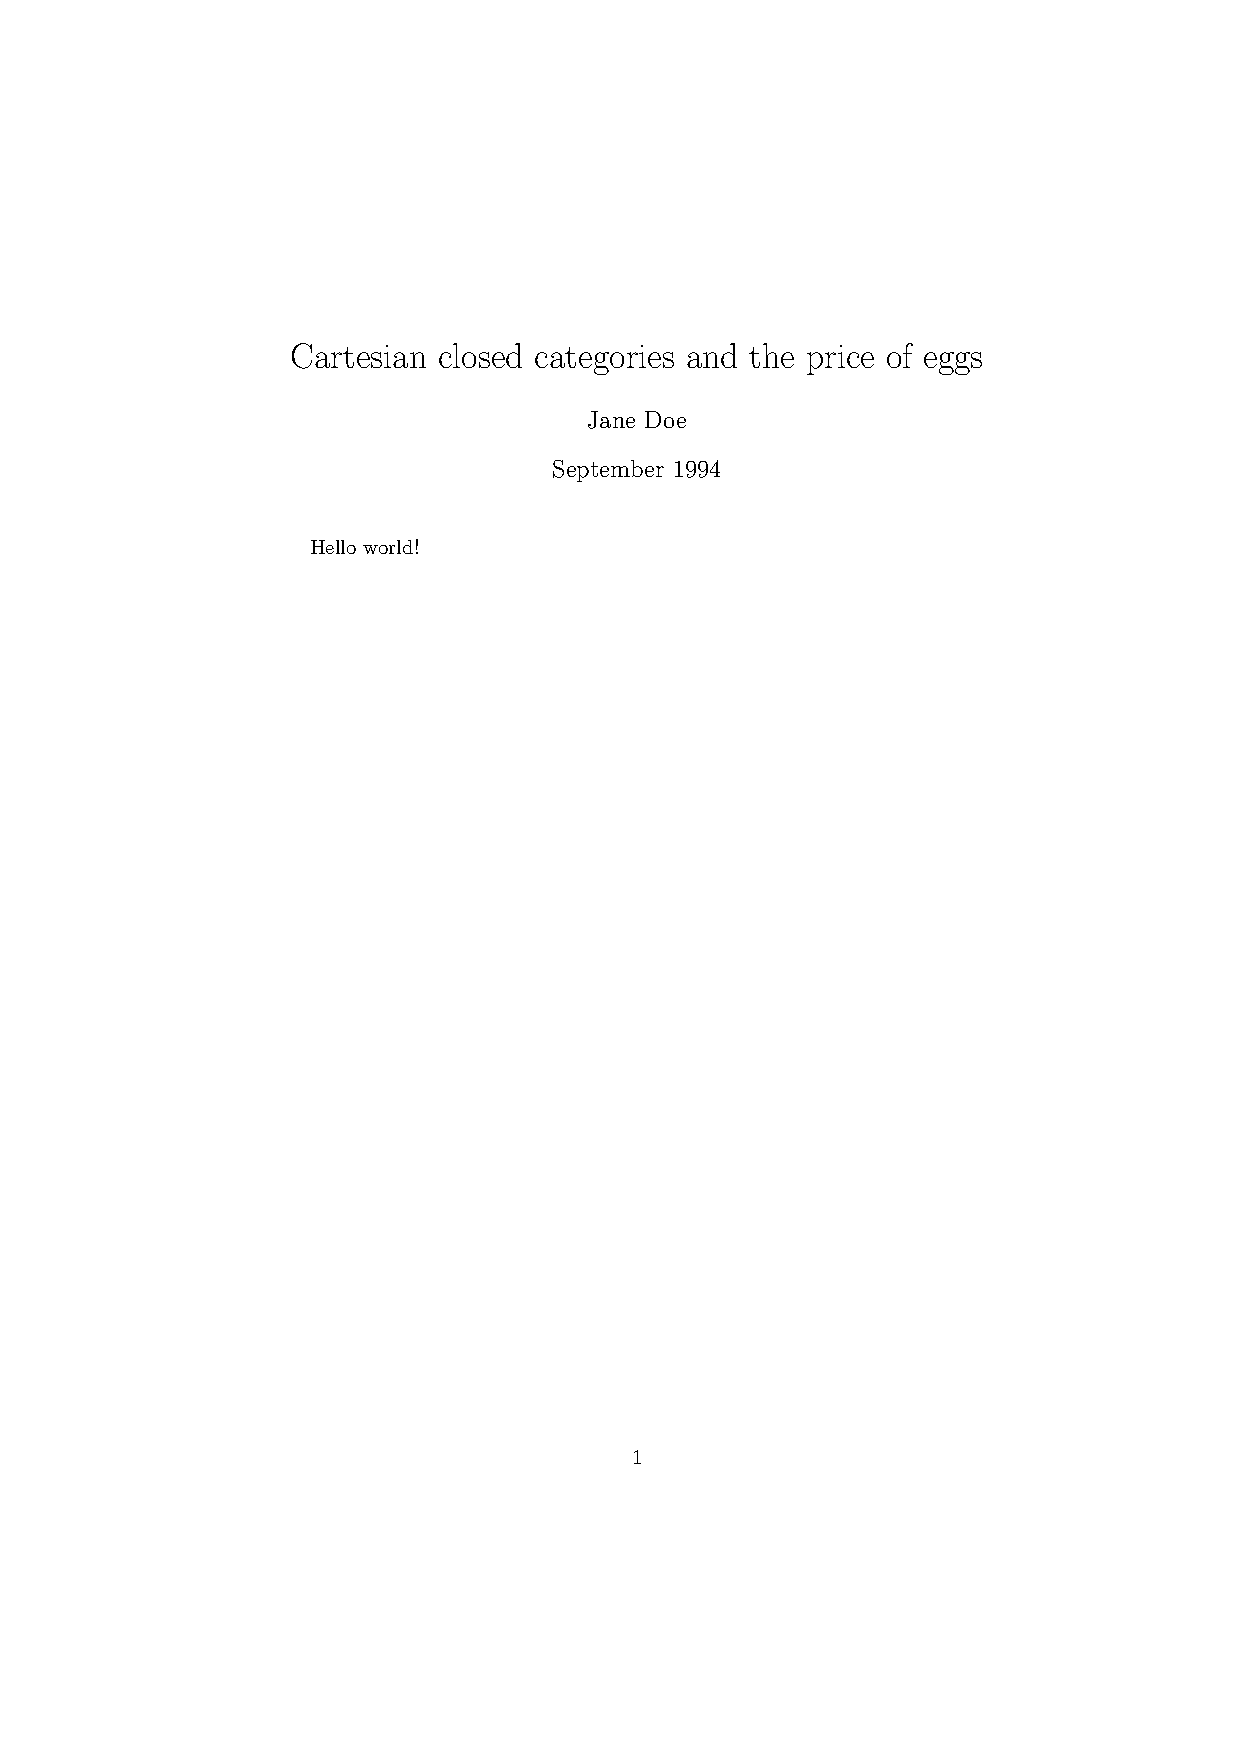
\includegraphics[trim = 1.5in 7in 1.5in 2in, clip, width = 4in]{hello}}
\end{frame}

\subsection{What is \LaTeX, anyway?}
\begin{frame}{\TeX}{...before \LaTeX}
  \begin{itemize}
    \item
      Typesetting system created by Donald Knuth
    \item
      Anybody could produce high-quality typography (in theory)
    \item
      Made to typeset complex mathematical formulae
    \item
      Popular in academic settings
    \item
      Difficulty and effort required gave rise to simplifications...
  \end{itemize}
\end{frame}

\begin{frame}{... enter \LaTeX}{``Lah-tech'' or ``Lay-tech'' as in Greek {$\tau\epsilon\chi$}}
  % - A title should summarize the slide in an understandable fashion
  %   for anyone how does not follow everything on the slide itself.

  \begin{itemize}
  \item
    Package of macros based on \TeX
  \item
    Created by Leslie Lamport
  \item
    Simplifies \TeX typesetting, especially for mathematical formulae
  \item
    Many additional packages and styles contributed by the community 
  \item
    Archived in the \hyperref[http://www.ctan.org]{Comprehensive TeX Archive Network (CTAN)}\footnote{http://www.ctan.org/}
  \end{itemize}
\end{frame}

\begin{frame}{The many facets of \LaTeX}
  \begin{itemize}
  \item {\LaTeX} refers to multiple things
  \item
    NOT a Word-Processor (e.g. Microsoft Word)
  \item
    WYSIWYM instead of WYSIWYG
  \begin{itemize}
    \item
      What-You-See-Is-What-You-Mean (semantics), versus
    \item
      What-You-See-Is-What-You-Get  (visual syntax)
  \end{itemize}
  \item
    Document Preparation System
  \begin{itemize}
    \item
      Made for high-quality typesetting
    \item
      Commonly used for technical/scientific documents
  \end{itemize}
  \item
    Document Markup Language
  \begin{itemize}
    \item
      Similar to HTML. (IMHO - could be better)
  \end{itemize}
  \end{itemize}
\end{frame}

\begin{frame}{Disadvantages}
  \begin{itemize}
  \item
    Lack of a 'Live Preview', must be compiled to view results.
    (This is general to all WYSIWYM systems.)
  \item
    Must learn the markup language and command syntax.
  \begin{itemize}
    \item
      Programmers feel right at home, but others may find this a
       difficulty in using \LaTeX
    \item
      Users only need to learn as much syntax as they want to use
    \item
      General to all markup languages
  \end{itemize}
  \item
    Difficult to manually adjust the typesetting
  \begin{itemize}
  \item
    This is frustrating to those familiar with WYSISYG editors
  \item
    This is actually considered an advantage by users familiar with
    \LaTeX
  \end{itemize}
  \end{itemize}
\end{frame}

\begin{frame}{Advantages}
  \begin{itemize}
  \item
    Forces authors to focus on the content (what you want to say)
      instead of the layout (how it looks on the page)
  \begin{itemize}
    \item
      This often trips up new users, who think of this as a
        requirement for document creation
  \end{itemize}
  \item
    The visual layout is consistent throughout a document
  \item
    Separation of content and style (like CSS on web pages)
    enables users to work on each seperately
  \item
    Mathematical Formulae (LaTeX is the standard)
  \item
    Indexes, ToC's, Footnotes, References and Bibliographies are
      easily and cleanly generated
  \begin{itemize}
    \item
      Compare to WYSIWYG editors
    \item
      Requires authors to correctly structure their documents
    \item
      Benefits the reader as well
  \end{itemize}
  \end{itemize}
\end{frame}

\subsection{How to use \LaTeX}

\begin{frame}{\LaTeX, the Document Creation System}
    \begin{figure}
        \begin{center}
        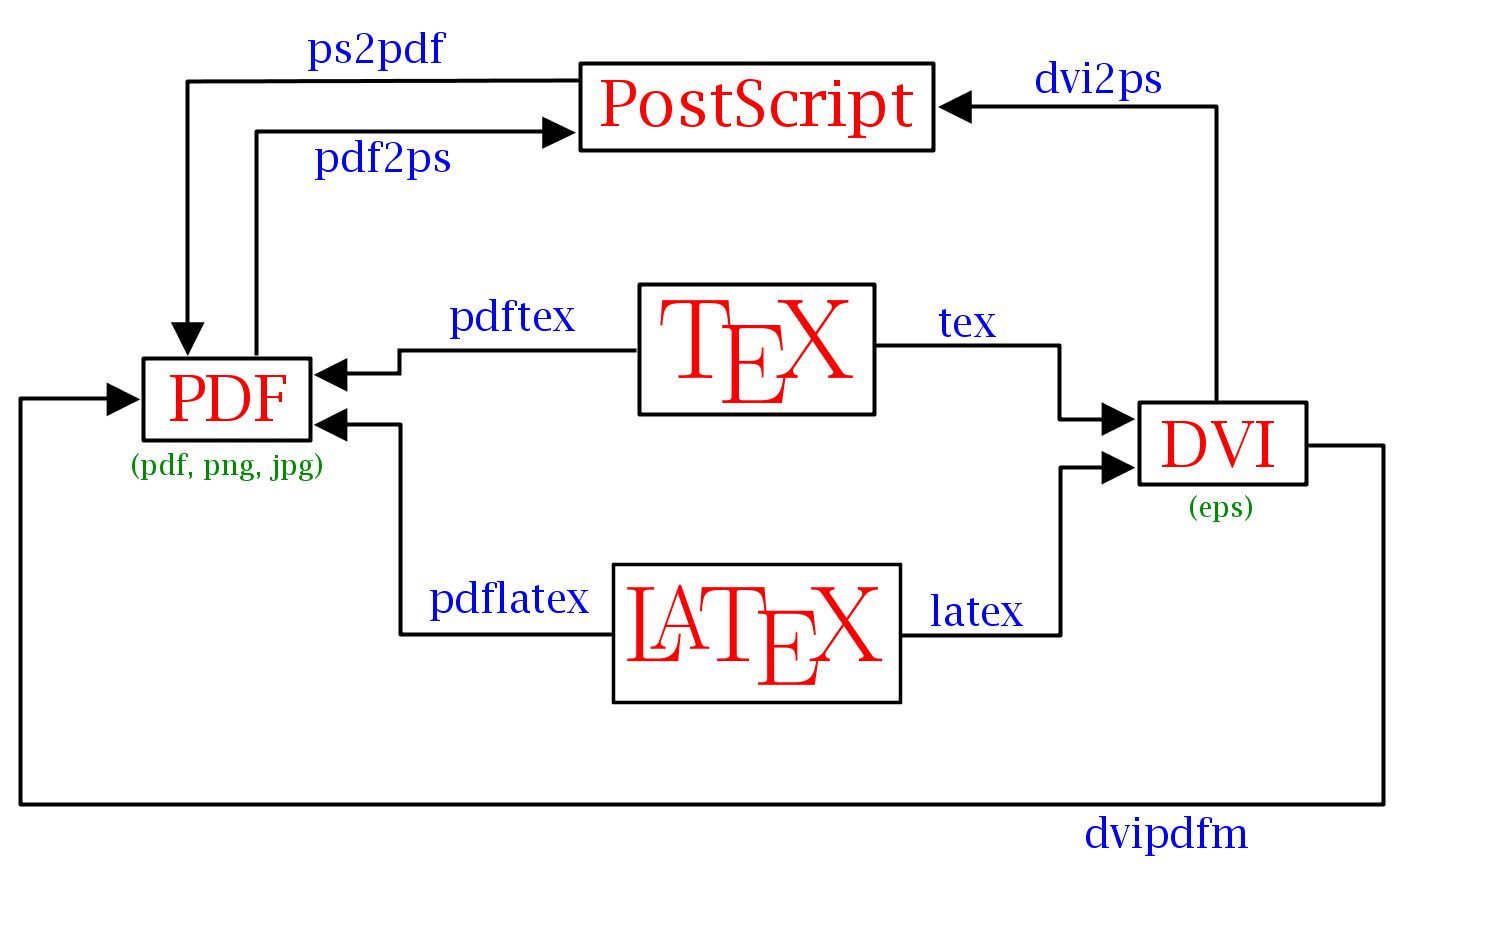
\includegraphics[width=0.9\textwidth]{LaTeXdiagram}
        \end{center}
    \end{figure}
\end{frame}

\begin{frame}{Simple Usage}
  \begin{itemize}
    \item
      The simplest usage case is using a general (raw) text editor:
    \begin{itemize}
      \item Examples: NotePad, Emacs, Vim, Notepad++, Wordpad
    \end{itemize}
    \item
      Documents are compiled via the command line
    \begin{itemize}
      \item Programs to compile .tex source:
        {\tt tex}, {\tt latex}, {\tt pdftex}, {\tt pdflatex}
      \item Programs to convert documents between types:
        {\tt dvi2ps}, {\tt ps2pdf}, {\tt pdf2ps}
    \end{itemize}
    \item
      Familiar approach to those that work in these (text) editors often
    \item
      Foreign approach to those used to WYSIWYG editors (everyone else)
  \end{itemize}
\end{frame}

\begin{frame}{Integrated Development Environments}
    \begin{itemize}
        \item Mac OS X
            \begin{itemize}
                \item \TeX shop -- \emph{http://www.uoregon.edu/~koch/texshop/}
            \end{itemize}
        \item Windows
            \begin{itemize}
                \item LEd (\LaTeX { Editor}) -- \emph{http://www.latexeditor.org}
                \item \TeX nicCenter -- \emph{http://www.texniccenter.org}
            \end{itemize}
        \item Linux
            \begin{itemize}
                \item Kile -- \emph{http://kile.sourceforge.net/}
            \end{itemize}
        \item Multiplatform
            \begin{itemize}
                \item \TeX maker -- \emph{http://www.xm1math.net/texmaker/}
                \item LyX -- WYSIWYM -- \emph{http://www.lyx.org/}
            \end{itemize}
    \end{itemize}
\end{frame}

\begin{frame}{Extending \LaTeX}
  \begin{itemize}
    \item
      Packages are sets of macros, commands, document classes, etc. that extend
      \LaTeX functionality past the base language.
    \item
      Examples include {\tt Beamer}-used to create this presentation, and
      {\tt AMSMath}-the ubiquitous Mathematics package.
    \item
      Huge number of packages available-all user contributed (karnaugh maps, finite state automata, analog circuit diagrams, ...)
    \item
      Usenet was the old go-to for \LaTeX packages, but has since become outdated.
    \item
      Use CTAN, the Comprehensive \TeX Archive Network. {\em http://www.ctan.org/}
    \item
      If you end up writing a set of useful \LaTeX macros, consider contributing them.
  \end{itemize}
\end{frame}

\subsection{The Language and Syntax}

\begin{frame}[fragile]{Syntax}
  \begin{itemize}
    \item
      Comments begin with `\%' and go to the end of the line
    \item
      Extend all the way through the next line's whitespace
    \item
      Commands begin with `\textbackslash'
    \begin{itemize}
      \item
        Optional Parameters go after command in []'s
      \item
        Required Parameters go after command in \{\}'s
      \item
        E.g. \verb|\cmdname[opt1,opt2,...]{arg1}{arg2}...|
    \end{itemize}
    \item
      Extra whitespace is ignored
    \item
      Environments are marked with \verb|\begin{}| and \verb|\end{}|
    \item
      Control Characters need to be escaped:
      \verb|\# \$ \% \^ \{ \} \& \_ \{ \} \~ \textbackslash|
  \end{itemize}
\end{frame}

\begin{frame}[containsverbatim]
    \frametitle{Text Formatting}
    \begin{itemize}
        \item Sizes: \begin{verbatim}\tiny, \scriptsize, \footnotesize, 
        \small, \normalsize, \large, \Large, \LARGE, \huge, \Huge\end{verbatim}
        \item \emph{Emphasis:} \verb|\emph{...}| {\em Also:} \verb|{\em ...}|
        \item Quotes: \LaTeX differentiates between ` and '.
        \begin{itemize}
            \item \verb|Single `quote'|: Single `quote'
            \item \verb|Double ``quote|: Double ``quote
        \end{itemize}
        \item Sub- and Superscript: \verb|\textsubscript{...}| and \verb|\textsuperscript{...}|
        \item {\bf Boldface} \verb|{\bf ...}|, {\it Italics} \verb|{\it ...}|, {\sc Small Caps} \verb|{\sc ..}| 
    \end{itemize}
\end{frame}

\begin{frame}[containsverbatim]
    \frametitle{Paragraph Formatting}
    \begin{itemize}
        \item Alignment:
            \begin{itemize}
                \item Left Justified: \verb|\begin{flushleft}| and \verb|\raggedleft|
                \item Right Justified: \verb|\begin(flushright}| and \verb|\raggedright|
                \item Centered: \verb|\begin{center}| and \verb|\centering|
            \end{itemize}
        \item Line Spacing:
            \begin{itemize}
                \item Entire Document: Use \verb|\linespread{...}| in the preamble. \verb|\linespread{1.3}| will yield \smash{\begin{math} 1 \frac{1}{2} \end{math}} line spacing, while \verb|\linespread{1.6}| will yield double.
                \item Section of Text: Include \verb|\usepackage{setspace}| in the preamble, which provides the \verb|singlespace|, \verb|onehalfspace|, \verb|doublespace| and \verb|spacing| environments.
                    \begin{itemize}
                    \item \verb|\begin{doublespace}| or \verb|\begin{spacing}{1.6}|
                    \end{itemize}
            \end{itemize}
    \end{itemize}
\end{frame}

\begin{frame}[containsverbatim]
    \frametitle{Verbatim and Lists}
    \begin{itemize}
        \item Verbatim: Outputs exactly what is typed
        \begin{itemize}
            \item \verb|\begin{verbatim}...\end{verbatim}|
        \end{itemize}
        \item Itemize:
        \begin{itemize}
            \item \verb|\begin{itemize}...\end{itemize}|
        \end{itemize}
        \item Enumerate:
        \begin{enumerate}
            \item \verb|\begin{enumerate}...\end{enumerate}|
        \end{enumerate}
        \item Description:
        \begin{description}
            \item[Environment Syntax:]  \verb|\begin{description}|
            \item[Item Syntax:] \verb|\item[Description]|
        \end{description}
        \item Each item is designated by the \verb|\item| command.
        \item Different list types can be nested.
    \end{itemize}
\end{frame}

\section{Examples}

\begin{frame}[containsverbatim]
    \frametitle{Math Environments}
    \begin{itemize}
        \item \LaTeX { uses} two different environments for mathematical formulae:
        \begin{itemize}
            \item \emph{text} -- Formulae are displayed in-line, within the body of text. Good for small equations.
            \begin{itemize}
                \item \verb|\begin{math}| \ldots \verb|\end{math}|
                \item (e.g.) \ldots thus arriving at \begin{math} a^2 + b^2 = c^2 \end{math}, which is the Pythagorean Theorem.
            \end{itemize}
            \item \emph{displayed} -- Formulae are displayed seperated from the text. Good for large equations.
            \begin{itemize}
            \item \verb|\begin{equation}| \ldots \verb|\end{equation}|
            \item (e.g.) \ldots which yields Stoke's Theorem: \begin{equation} \int_\Sigma \nabla \times \mathbf{F} \cdot \mathrm{d}\Sigma = \oint_{\partial\Sigma} \mathbf{F} \cdot \mathrm{d}\mathbf{r} \end{equation}
            \end{itemize}
        \end{itemize}
    \item Always include the amsmath package by using the command \verb|\usepackage{amsmath}|.
    \end{itemize}
\end{frame}

\subsection{Floats, Figures, Tables}

\begin{frame}[containsverbatim]
    \frametitle{Figures}
        \begin{itemize}
        \item When compiling with \emph{latex}, only Encapsulated Postscript (EPS) files can be imported.
        \item Compiling with \emph{pdflatex} allows JPG, PDF, and PNG formats to be imported.
        \item By using the \verb|draft| option in the \verb|\documentclass[...]{...}| command in the preamble, image output can be suppressed and every image will be replaced by the name of that image.
        \item Remember to include the command \verb|\usepackage{graphicx}|.
        \item Use floats! (\verb|\begin{figure}| and \verb|\begin{table}|)
    \end{itemize}
\end{frame}

\begin{frame}[containsverbatim]
    \frametitle{Figures by Example}
    \begin{figure}
        \begin{center}
        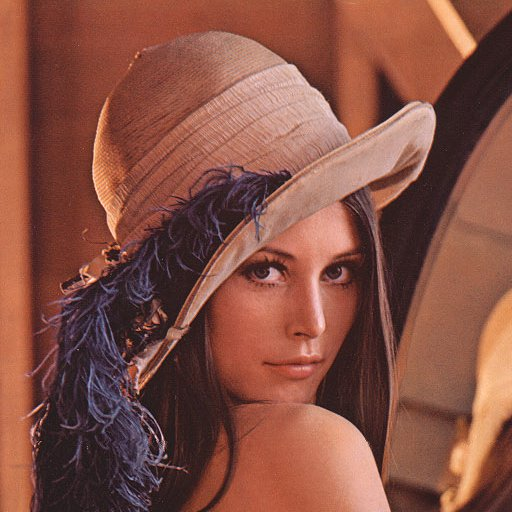
\includegraphics[width=0.3\textwidth]{lena.jpg}
        \end{center}
    \end{figure}

    \begin{block}{\LaTeX{ }Code:}
    \begin{verbatim}
        \begin{figure}
        \begin{center}
        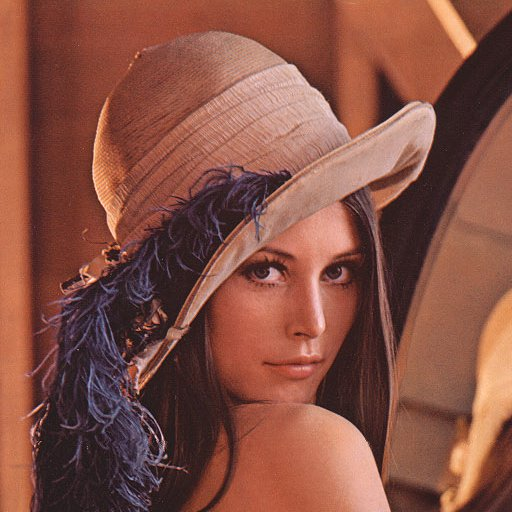
\includegraphics[width=0.3\textwidth]{lena.jpg}
        \end{center}
        \end{figure}
    \end{verbatim}
    \end{block}
\end{frame}

\begin{frame}[containsverbatim]
    \frametitle{Figures by Example}
    \begin{figure}
        \begin{center} \vspace{-10pt}
            \reflectbox{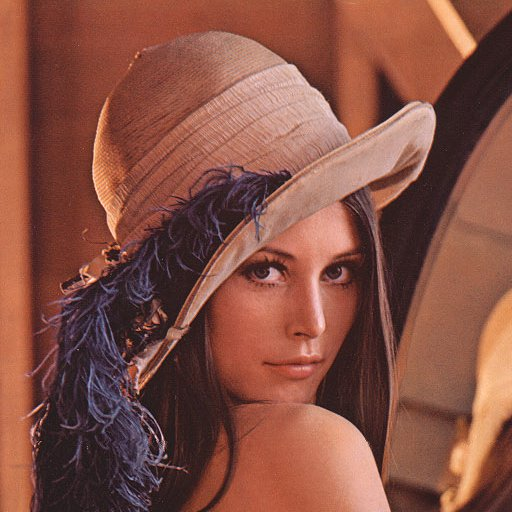
\includegraphics[scale=0.1, angle = -15]{lena.jpg}}
            \label{CNematic}
            \caption{A Liquid Crystal} \vspace{-15pt}
        \end{center}
    \end{figure}

    \begin{block}{\LaTeX{ }Code:}
    \scriptsize{
    \begin{verbatim}
    \begin{figure}[h] %t, b, p, !, and H (with \usepackage{float})
        \begin{center} \vspace{-5pt}
            \reflectbox{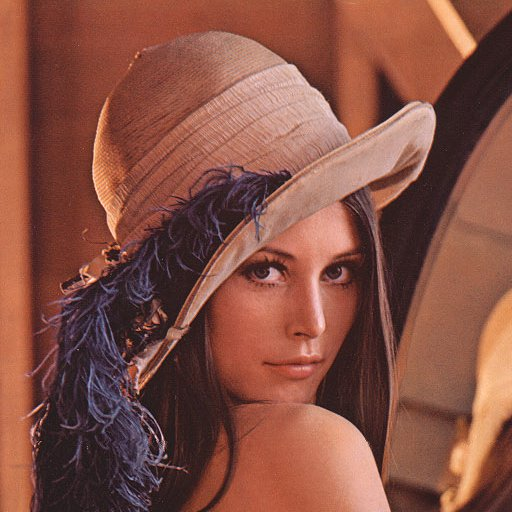
\includegraphics[scale=0.1, angle = -15]{lena.jpg}}
            \label{CNematic}
            \caption{A Liquid Crystal} \vspace{-10pt}
        \end{center}
    \end{figure}
    \end{verbatim}}
    \end{block} 
\end{frame}

\begin{frame}[containsverbatim]
    \frametitle{Tables by Example}
    \begin{table}
        \begin{tabular}[c]{|l || c | c | c | c |}
            \hline
                Component & Target (\%) & Target (g) & Actual (g) & Actual(\%) \\
            \hline
                RMS03-010C & 98.2 \% & .5024 g & .5032 g & 98.4 \% \\
            \hline
        \end{tabular}
        \label{tab:measure}
        \caption{A Table of Measurements}
        \vspace{-15pt}
    \end{table}

    \begin{block}{\LaTeX{ }Code:}
    \footnotesize{
    \begin{verbatim}
    \begin{table}
        \begin{tabular}[c]{|l || c | c | c | c |}
            \hline
                Component & Target (\%) & Target (g) & Actual (g) & Actual(\%) \\
            \hline
                RMS03-010C & 98.2 \% & .5024 g & .5032 g & 98.4 \% \\
            \hline
        \end{tabular}
    \caption{A Table of Measurements}
    \label{tab:measure}
    \end{table}
    \end{verbatim}}
    \end{block} 
\end{frame}

\begin{frame}[containsverbatim]
    \frametitle{Referencing Labels}
    \begin{itemize}
    \item As seen before, an object can be labeled by using the \verb|\label{...}| command. 
    \item This object can be referenced using this label with the command \verb|\ref{...}|. This will print the number assigned to the object.
    \item Similarly, \verb|\pageref{...}| will print the page number of the referenced object.
    \item Be sure to use \verb|\label{...}| \emph{after} \verb|\caption{...}|. Otherwise, the reference will be attached to the current section or list number.
    \item Lists of Tables and Lists of Figures can be created by using \verb|\listoftables| or \verb|\listoffigures|. This will create a numerically ordered list of floats, complete with captions.
    \item The caption command allows for both short captions and long captions. This is done by using \verb|\caption[short comment]{long comment}|.
    \end{itemize}
\end{frame}

\subsection{Other examples}
\begin{frame}{Presentation fun}

  You can create overlays\dots
  \begin{itemize}
  \item using the \texttt{pause} command:
    \begin{itemize}
    \item
      First item.
      \pause
    \item    
      Second item.
    \end{itemize}
  \item
    using overlay specifications:
    \begin{itemize}
    \item<3->
      First item.
    \item<4->
      Second item.
    \end{itemize}
  \item
    using the general \texttt{uncover} command:
    \begin{itemize}
      \uncover<5->{\item
        First item.}
      \uncover<6->{\item
        Second item.}
    \end{itemize}
  \end{itemize}
\end{frame}


\section*{Questions?}

\begin{frame}{Any Questions?}
  This presentation will be posted online for reference.\\
  
  \LaTeX is much too large a topic to cover in one sitting, but hopefully this is a good start.\\
  
  Other References:
  \begin{itemize}
    \item \href{http://en.wikipedia.org/wiki/LaTeX}{Wikipedia article on \LaTeX}
    \item \href{http://www.latex-project.org/}{\LaTeX{ }Project Site}
    \item \href{http://en.wikibooks.org/wiki/LaTeX/}{Wikibook on \LaTeX}
  \end{itemize}
\end{frame}



\section*{Summary}

\begin{frame}{Summary}

  % Keep the summary *very short*.
  \begin{itemize}
  \item
    The \alert{first main message} of your talk in one or two lines.
  \item
    The \alert{second main message} of your talk in one or two lines.
  \item
    Perhaps a \alert{third message}, but not more than that.
  \end{itemize}
  
  % The following outlook is optional.
  \vskip0pt plus.5fill
  \begin{itemize}
  \item
    Outlook
    \begin{itemize}
    \item
      Something you haven't solved.
    \item
      Something else you haven't solved.
    \end{itemize}
  \end{itemize}
\end{frame}



% All of the following is optional and typically not needed. 
\appendix
\section<presentation>*{\appendixname}
\subsection<presentation>*{For Further Reading}

\begin{frame}[allowframebreaks]
  \frametitle<presentation>{For Further Reading}
    
  \begin{thebibliography}{10}
    
  \beamertemplatebookbibitems
  % Start with overview books.

  \bibitem{Author1990}
    A.~Author.
    \newblock {\em Handbook of Everything}.
    \newblock Some Press, 1990.
 
    
  \beamertemplatearticlebibitems
  % Followed by interesting articles. Keep the list short. 

  \bibitem{Someone2000}
    S.~Someone.
    \newblock On this and that.
    \newblock {\em Journal of This and That}, 2(1):50--100,
    2000.
  \end{thebibliography}
\end{frame}

\end{document}
